% IEEE conference paper. Build: `make paper` (numbers, tables and figures are generated from the
% recorded evaluation by experiments/paper_build.py: no result below is typed by hand), or compile
% this folder on Overleaf (generated/ and figures/ are included).
\documentclass[conference]{IEEEtran}
\IEEEoverridecommandlockouts
\usepackage{cite}
\usepackage{amsmath,amssymb,amsfonts}
\usepackage{algorithm}
\usepackage{algorithmic}
\usepackage{graphicx}
\usepackage{textcomp}
\usepackage{xcolor}
\usepackage{booktabs}
\usepackage{url}
\usepackage{tikz}
\usetikzlibrary{positioning,arrows.meta,calc}
% pdfLaTeX (Overleaf) sets Times through IEEEtran; XeTeX (Tectonic, `make paper`) needs it named.
\ifx\XeTeXversion\undefined\else
  \usepackage[T1]{fontenc}
\fi
% Generated by experiments/paper_build.py from the recorded evaluation. Do not edit.
\newcommand{\AnoDelayCochan}{25}
\newcommand{\AnoDelayFail}{5}
\newcommand{\AnoF}{0.964}
\newcommand{\AnoPrecision}{0.950}
\newcommand{\AnoRecall}{0.979}
\newcommand{\CfgBaseLatency}{0.8}
\newcommand{\CfgBaseLoss}{0.2}
\newcommand{\CfgBulk}{0.394}
\newcommand{\CfgCapacity}{4.6}
\newcommand{\CfgChangePct}{5}
\newcommand{\CfgCochanFull}{30}
\newcommand{\CfgCochanZero}{60}
\newcommand{\CfgFetch}{0.8}
\newcommand{\CfgForestSeed}{42}
\newcommand{\CfgHighImpactGap}{120}
\newcommand{\CfgLatCap}{15.8}
\newcommand{\CfgMaxActions}{3}
\newcommand{\CfgMaxSteerPct}{30}
\newcommand{\CfgMinRssi}{-75}
\newcommand{\CfgPeriod}{5}
\newcommand{\CfgQueueSlots}{6}
\newcommand{\CfgRegressPct}{10}
\newcommand{\CfgServiceMs}{2.5}
\newcommand{\CfgSettle}{10}
\newcommand{\CfgStationSeed}{7}
\newcommand{\CfgTxStep}{3}
\newcommand{\CfgUtilHigh}{0.8}
\newcommand{\CfgUtilTarget}{0.6}
\newcommand{\CfgWatch}{30}
\newcommand{\FairJainVone}{0.51}
\newcommand{\FairJainVthree}{0.79}
\newcommand{\FairJainVtwo}{0.78}
\newcommand{\FcHoltOne}{0.129}
\newcommand{\FcHoltThree}{0.256}
\newcommand{\FcMaOne}{0.117}
\newcommand{\FcMaThree}{0.212}
\newcommand{\GenActions}{6}
\newcommand{\GenActionsVerdict}{6}
\newcommand{\GenCopilotN}{5}
\newcommand{\GenCopilotOk}{5}
\newcommand{\GenRcaN}{3}
\newcommand{\GenRcaOk}{3}
\newcommand{\HarmAccepted}{21}
\newcommand{\HarmAll}{23}
\newcommand{\HarmAnyRegress}{11}
\newcommand{\HarmFisherP}{0.32}
\newcommand{\HarmJainOnly}{1}
\newcommand{\HarmRejected}{2}
\newcommand{\HarmVthree}{20}
\newcommand{\HoneCapped}{not met}
\newcommand{\HoneFasterApFail}{17}
\newcommand{\HoneFasterCochan}{0}
\newcommand{\HoneFasterFlash}{8}
\newcommand{\HoneVerdictApFail}{inconclusive}
\newcommand{\HoneVerdictCochan}{inconclusive}
\newcommand{\HoneVerdictFlash}{inconclusive}
\newcommand{\IntCalls}{60}
\newcommand{\IntCases}{30}
\newcommand{\IntCloudOk}{30}
\newcommand{\IntCloudSeconds}{2.0}
\newcommand{\IntFirstValid}{60}
\newcommand{\IntLocalOk}{21}
\newcommand{\IntLocalSeconds}{2.5}
\newcommand{\IntRepairs}{0}
\newcommand{\KeptAll}{38}
\newcommand{\KpiApFailJainVone}{0.96}
\newcommand{\KpiApFailJainVthree}{0.89}
\newcommand{\KpiApFailJainVtwo}{0.91}
\newcommand{\KpiApFailLatVone}{18}
\newcommand{\KpiApFailLatVthree}{672}
\newcommand{\KpiApFailLatVtwo}{348}
\newcommand{\KpiApFailLossVone}{4.8}
\newcommand{\KpiApFailLossVthree}{18.8}
\newcommand{\KpiApFailLossVtwo}{10.0}
\newcommand{\KpiApFailThrVone}{0.64}
\newcommand{\KpiApFailThrVthree}{0.58}
\newcommand{\KpiApFailThrVtwo}{0.84}
\newcommand{\KpiApFailTtrVone}{360}
\newcommand{\KpiApFailTtrVthree}{300}
\newcommand{\KpiApFailTtrVtwo}{142}
\newcommand{\KpiCochanJainVone}{0.93}
\newcommand{\KpiCochanJainVthree}{0.94}
\newcommand{\KpiCochanJainVtwo}{0.95}
\newcommand{\KpiCochanLatVone}{11}
\newcommand{\KpiCochanLatVthree}{11}
\newcommand{\KpiCochanLatVtwo}{22}
\newcommand{\KpiCochanLossVone}{48.2}
\newcommand{\KpiCochanLossVthree}{25.7}
\newcommand{\KpiCochanLossVtwo}{9.1}
\newcommand{\KpiCochanThrVone}{0.18}
\newcommand{\KpiCochanThrVthree}{0.31}
\newcommand{\KpiCochanThrVtwo}{0.60}
\newcommand{\KpiCochanTtrVone}{420}
\newcommand{\KpiCochanTtrVthree}{420}
\newcommand{\KpiCochanTtrVtwo}{146}
\newcommand{\KpiFlashJainVone}{0.51}
\newcommand{\KpiFlashJainVthree}{0.79}
\newcommand{\KpiFlashJainVtwo}{0.78}
\newcommand{\KpiFlashLatVone}{21}
\newcommand{\KpiFlashLatVthree}{25}
\newcommand{\KpiFlashLatVtwo}{24}
\newcommand{\KpiFlashLossVone}{43.9}
\newcommand{\KpiFlashLossVthree}{8.5}
\newcommand{\KpiFlashLossVtwo}{9.2}
\newcommand{\KpiFlashThrVone}{0.20}
\newcommand{\KpiFlashThrVthree}{0.53}
\newcommand{\KpiFlashThrVtwo}{0.52}
\newcommand{\KpiFlashTtrVone}{390}
\newcommand{\KpiFlashTtrVthree}{359}
\newcommand{\KpiFlashTtrVtwo}{374}
\newcommand{\LedVoneKept}{0}
\newcommand{\LedVoneProposed}{0}
\newcommand{\LedVoneRejected}{0}
\newcommand{\LedVoneRollbackFailed}{0}
\newcommand{\LedVoneRolledBack}{0}
\newcommand{\LedVoneWaiting}{0}
\newcommand{\LedVoneWatched}{0}
\newcommand{\LedVthreeKept}{33}
\newcommand{\LedVthreeProposed}{65}
\newcommand{\LedVthreeRejected}{4}
\newcommand{\LedVthreeRollbackFailed}{2}
\newcommand{\LedVthreeRolledBack}{18}
\newcommand{\LedVthreeWaiting}{8}
\newcommand{\LedVthreeWatched}{0}
\newcommand{\LedVtwoKept}{38}
\newcommand{\LedVtwoProposed}{64}
\newcommand{\LedVtwoRejected}{0}
\newcommand{\LedVtwoRollbackFailed}{1}
\newcommand{\LedVtwoRolledBack}{22}
\newcommand{\LedVtwoWaiting}{0}
\newcommand{\LedVtwoWatched}{3}
\newcommand{\LiveJainBase}{2.7}
\newcommand{\LiveJainErr}{0.0}
\newcommand{\LiveJainN}{114}
\newcommand{\LiveLatBase}{62.3}
\newcommand{\LiveLatErr}{70.5}
\newcommand{\LiveLatN}{114}
\newcommand{\LiveLossBase}{50.3}
\newcommand{\LiveLossErr}{57.2}
\newcommand{\LiveLossN}{102}
\newcommand{\LiveN}{114}
\newcommand{\LiveThrBase}{46.5}
\newcommand{\LiveThrErr}{56.7}
\newcommand{\LiveThrN}{114}
\newcommand{\NeverApFailVone}{3}
\newcommand{\NeverApFailVthree}{2}
\newcommand{\NeverApFailVtwo}{1}
\newcommand{\NeverCochanVone}{3}
\newcommand{\NeverCochanVthree}{3}
\newcommand{\NeverCochanVtwo}{0}
\newcommand{\NeverFlashVone}{3}
\newcommand{\NeverFlashVthree}{1}
\newcommand{\NeverFlashVtwo}{2}
\newcommand{\NumRuns}{27}
\newcommand{\PerSeedLatApFailVthree}{15, 1000, 1000}
\newcommand{\PerSeedLatApFailVtwo}{1000, 24, 21}
\newcommand{\PerSeedLossApFailVthree}{4.2, 26.1, 26.0}
\newcommand{\PerSeedLossApFailVtwo}{25.2, 2.7, 2.3}
\newcommand{\RbFailAll}{3}
\newcommand{\RbFailApFail}{3}
\newcommand{\RecovVone}{0}
\newcommand{\RecovVthree}{3}
\newcommand{\RecovVtwo}{6}
\newcommand{\RuleAgree}{114}
\newcommand{\RuleConjHarm}{4}
\newcommand{\RuleConjKept}{6}
\newcommand{\RuleNoRegHarm}{4}
\newcommand{\RuleNoRegKept}{4}
\newcommand{\RuleTotal}{114}
\newcommand{\RuleWrittenHarm}{2}
\newcommand{\RuleWrittenKept}{1}
\newcommand{\SafeVoneApplied}{0}
\newcommand{\SafeVoneAppliedTwinRejected}{0}
\newcommand{\SafeVoneHarmfulTwinRejected}{0}
\newcommand{\SafeVoneHighImpactUnapproved}{0}
\newcommand{\SafeVoneRecorded}{0}
\newcommand{\SafeVoneRollbackFailed}{0}
\newcommand{\SafeVoneSlippedPastTwin}{0}
\newcommand{\SafeVoneUnresolved}{0}
\newcommand{\SafeVthreeApplied}{53}
\newcommand{\SafeVthreeAppliedTwinRejected}{0}
\newcommand{\SafeVthreeHarmfulTwinRejected}{0}
\newcommand{\SafeVthreeHighImpactUnapproved}{0}
\newcommand{\SafeVthreeRecorded}{65}
\newcommand{\SafeVthreeRollbackFailed}{2}
\newcommand{\SafeVthreeSlippedPastTwin}{18}
\newcommand{\SafeVthreeUnresolved}{0}
\newcommand{\SafeVtwoApplied}{64}
\newcommand{\SafeVtwoAppliedTwinRejected}{3}
\newcommand{\SafeVtwoHarmfulTwinRejected}{2}
\newcommand{\SafeVtwoHighImpactUnapproved}{9}
\newcommand{\SafeVtwoRecorded}{64}
\newcommand{\SafeVtwoRollbackFailed}{1}
\newcommand{\SafeVtwoSlippedPastTwin}{20}
\newcommand{\SafeVtwoUnresolved}{3}
\newcommand{\SimMedianMs}{0.61}
\newcommand{\TwinBulkHigh}{21}
\newcommand{\TwinBulkLow}{12}
\newcommand{\TwinChannel}{8.1}
\newcommand{\TwinChannelN}{10}
\newcommand{\TwinMape}{4.5}
\newcommand{\TwinN}{586}
\newcommand{\TwinSteadyN}{495}
\newcommand{\TwinSteadyVideo}{4.0}
\newcommand{\TwinSteer}{3.3}
\newcommand{\VtwoAccHarm}{21}
\newcommand{\VtwoAccTotal}{58}
\newcommand{\VtwoRejHarm}{2}
\newcommand{\VtwoRejTotal}{3}


\newcommand{\KPI}{\mathbf{k}}
\newcommand{\pct}[1]{#1\%}

\begin{document}

\title{A Twin-Gated Control Loop for Campus Wi-Fi:\\ Verifying SDN and LLM-Proposed Actions in a Digital Twin Before They Reach the Network}

\author{
\IEEEauthorblockN{Aggimalla Abhishek, N. Likhith Naik, Sundaram, Sambhav Mishra, Bikram Hawaldar}
\IEEEauthorblockA{Indian Institute of Information Technology Dharwad, India}
\and
\IEEEauthorblockN{Jagadeesha R B}
\IEEEauthorblockA{Dept.\ of Electronics and Communication Engineering\\
Indian Institute of Information Technology Dharwad, India}
}

\maketitle

\begin{abstract}
A software-defined network (SDN) controller can react to congestion, access-point (AP) failures and interference in campus Wi-Fi, but a change applied directly to the live network shows its effect only afterwards. We present a control loop in which no action, whether proposed by a heuristic optimizer or by a large language model (LLM) that translates an operator's intent, reaches the network without an accepted verdict from a digital twin. The twin is an analytical model of per-AP airtime sharing, co-channel interference and M/M/1/K queueing. An executor applies accepted actions, watches the live KPIs and rolls back regressions. On an emulated campus (Mininet-WiFi and Ryu; 4 APs, 20 stations) we compare plain SDN (V1), heuristics without the twin (V2) and the full system (V3) in three scenarios and three seeds each (\NumRuns{} runs). The twin predicts per-flow throughput within \TwinMape\% and answers in a median \SimMedianMs\,ms. In a lecture flash crowd both acting variants cut the loss of the affected flows from \KpiFlashLossVone\% to under 10\% and more than double their throughput. The hypothesis that V3 recovers 30\% faster than V1 stays inconclusive, because plain SDN never recovered. The twin rejected few actions: most harmful ones were accepted, and the watch-and-rollback step, which itself failed \RbFailAll{} times, gave the main protection. An LLM behind schema validation translated \IntCloudOk{} of \IntCases{} test intents correctly. We report these negative results together with the code, data and scripts that reproduce them.
\end{abstract}

\begin{IEEEkeywords}
digital twin, software-defined networking, Wi-Fi, large language models, intent-based networking, safe automation
\end{IEEEkeywords}

\section{Introduction}
Campus Wi-Fi is never still: students move between rooms, a lecture fills a hall within minutes, an AP fails, and neighbouring APs on one channel slow each other down. An SDN controller can react by steering clients to a less loaded AP, changing an AP's channel or prioritizing a traffic class. Reacting is risky, because a controller that applies a change directly learns its effect only afterwards, and the risk grows as more decisions are automated, whether by an optimizer or by an LLM that turns a goal such as ``video calls in the lab must stay smooth'' into policy. LLM output can be wrong, incomplete or unsafe, and nothing checks it before it takes effect.

We make a \emph{digital twin} of the network the gate that every change must pass. The twin mirrors the live state from telemetry and predicts the effect of a candidate action on throughput, latency, loss and fairness before it is applied. We ask whether this makes an AI-driven controller both more effective and safer than acting directly, and whether an LLM can drive it from natural language. We test three hypotheses:
\textbf{H1}~the full system (V3) recovers from congestion at least 30\% faster than plain SDN (V1);
\textbf{H2}~the twin blocks actions that would hurt the KPIs and that an optimizer acting directly (V2) would apply;
\textbf{H3}~an LLM with schema-constrained output translates at least 20 of 30 intents correctly, and no invalid configuration reaches the network.

\emph{Contributions.}
(i)~A reproducible, fully virtual wireless SDN testbed with seeded campus scenarios and an explicit model of co-channel interference, which the emulator does not produce itself.
(ii)~An analytical twin of airtime sharing and queueing, validated against the testbed, fast enough for a 5\,s control loop.
(iii)~A closed loop (propose, verify, apply, watch, roll back) in which the twin's accepted verdict is enforced in the code that applies changes.
(iv)~An LLM intent pipeline in which the model only translates text into a validated policy; deterministic code compiles it into bounded actions.
(v)~An evaluation of three controllers over \NumRuns{} runs that reports what did not work.

\section{Related Work}
\emph{Network digital twins.} Almasan et al.\ \cite{almasan2022} describe the network digital twin as an accurate, data-driven model of a real network, used chiefly to answer ``what if'' questions before a change. We share the split between a mirror of the live state and a performance model, but our model is analytical, needs no training data and can be explained, and we use the twin as a \emph{safety gate}: no action is applied without its accepted verdict.
\emph{Learned performance models.} RouteNet \cite{rusek2020} uses a graph neural network to predict per-path delay, jitter and loss and to score routing candidates. We follow its use of a fast model inside the loop and its relative-error reporting, but our bottleneck is the shared Wi-Fi medium, which we model explicitly; a learned surrogate is future work.
\emph{LLM-based intent networking.} Mekrache et al.\ \cite{mekrache2024} manage the intent life cycle in natural language on a 5G testbed. We adopt natural language as the operator interface, but trust the model less: its output must pass a JSON schema, is compiled by deterministic code and is simulated in the twin, and the model has no tool that changes the network.
\emph{Programmable WLANs.} Odin \cite{suresh2012} makes enterprise WLANs programmable through a per-client virtual AP, because clients, not the infrastructure, choose their AP. We steer clients by explicit re-association, which costs a reconnection that the twin accounts for.
\emph{Emulation.} We build on Mininet \cite{lantz2010}, Mininet-WiFi \cite{fontes2015} and OpenFlow \cite{mckeown2008} with the Ryu controller.
None of these works combines a wireless twin, natural-language control and a verification step before every action.

\section{Problem Scenario and System Model}
\subsection{Scenario}
The campus has four zones, each served by one AP: a lecture hall (ap1, channel 1), a lab (ap2, channel 6), a corridor (ap3, channel 11) and a library (ap4, channel 1), two OpenFlow switches and 20 stations carrying video, web and bulk traffic. ap1 and ap4 share channel 1 but are 50\,m apart. An AP carries about \CfgCapacity\,Mbit/s downlink on our testbed. Each 600\,s scenario has one disruption: a \emph{lecture flash crowd} (ten students walk into the hall from 120\,s, video starts at 210\,s), an \emph{AP failure} (ap2 goes down at 240\,s) and \emph{co-channel interference} (ap3 is forced onto channel 1 at 180\,s). The problem is to restore service quickly using only allow-listed actions, without making things worse for users.

\subsection{System model}
Fig.~\ref{fig:arch} shows the architecture. The testbed streams AP, station and flow telemetry to a time-series store. The twin rebuilds its state $s$ from the last 10\,s of telemetry at each refresh (no accumulated state, so it cannot drift from the network); an AP silent for 5\,s counts as down. The state holds every AP (position, channel, up/down, utilization), station (AP, zone) and flow (measured throughput, latency, loss, queue, rate limit).

\begin{figure}[t]
\centering
\resizebox{\columnwidth}{!}{%
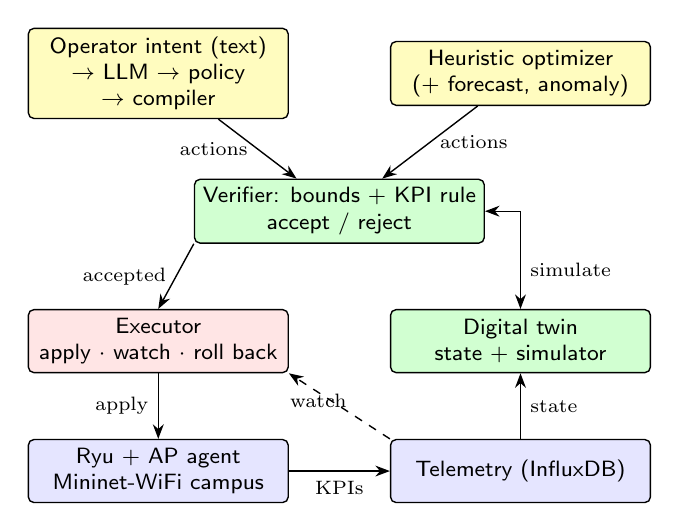
\begin{tikzpicture}[font=\sffamily\footnotesize, >=Stealth, line width=0.5pt,
  box/.style={draw, rounded corners=2pt, align=center, inner sep=3pt, minimum height=8mm},
  prop/.style={box, fill=yellow!25}, gate/.style={box, fill=green!18},
  net/.style={box, fill=blue!10}, act/.style={box, fill=red!10}]
\node[prop, minimum width=33mm] (llm) at (0,3.1) {Operator intent (text)\\$\rightarrow$ LLM $\rightarrow$ policy\\$\rightarrow$ compiler};
\node[prop, minimum width=33mm] (opt) at (4.6,3.1) {Heuristic optimizer\\(+ forecast, anomaly)};
\node[gate, minimum width=33mm] (ver) at (2.3,1.35) {Verifier: bounds + KPI rule\\accept / reject};
\node[gate, minimum width=33mm] (twin) at (4.6,-0.3) {Digital twin\\state + simulator};
\node[act, minimum width=33mm] (exe) at (0,-0.3) {Executor\\apply $\cdot$ watch $\cdot$ roll back};
\node[net, minimum width=33mm] (net) at (0,-1.95) {Ryu + AP agent\\Mininet-WiFi campus};
\node[net, minimum width=33mm] (db) at (4.6,-1.95) {Telemetry (InfluxDB)};
\draw[->] (llm) -- node[left, font=\scriptsize]{actions} (ver);
\draw[->] (opt) -- node[right, font=\scriptsize]{actions} (ver);
\draw[<->] (ver.east) -| node[right, pos=0.8, font=\scriptsize]{simulate} (twin.north);
\draw[->] (ver.south west) -- node[left, font=\scriptsize]{accepted} (exe.north);
\draw[->] (exe) -- node[left, font=\scriptsize]{apply} (net);
\draw[->] (net) -- node[below, font=\scriptsize]{KPIs} (db);
\draw[->] (db) -- node[right, font=\scriptsize]{state} (twin);
\draw[->, dashed] (db.north west) -- node[above left=-1pt, font=\scriptsize, pos=0.35]{watch} (exe.south east);
\end{tikzpicture}}
\caption{Architecture. Proposals come from a heuristic optimizer or from an LLM-compiled policy. Only actions that the verifier accepts reach the executor, the only component that changes the network.}
\label{fig:arch}
\end{figure}

An \emph{action} $a$ is one of seven allow-listed types (reroute, QoS queue, rate limit, client steering, transmit power, channel change, AP admin state), each with an impact class. QoS and rerouting (low impact) and client steering (medium impact, validated against the testbed) are applied when the twin accepts them; the other medium-impact types (rate limit, transmit power) wait for an operator until their predictions are validated; a channel change or taking an AP down is \emph{high impact} and always waits for an operator. The measured KPI vector of a set of flows is $\KPI=(T,L_{95},\bar\ell,J)$: mean throughput, 95th-percentile video latency, mean loss and Jain's fairness index \cite{jain1984} of the APs' client counts.

\section{Mathematical Formulation}
\subsection{Analytical twin}
\emph{Capacity.} An AP $i$ that is up offers $C=\CfgCapacity$\,Mbit/s, reduced by every up AP $j\neq i$ on its channel:
\begin{equation}
C_i=\frac{C}{1+\sum_{j\neq i,\ \mathrm{ch}(j)=\mathrm{ch}(i)} w(d_{ij})},
\label{eq:cap}
\end{equation}
where $d_{ij}$ is the distance between the APs, $w(d)=\min\{1,\max\{0,(d_2-d)/(d_2-d_1)\}\}$, $d_1=\CfgCochanFull$\,m (a same-channel AP this close takes a full share) and $d_2=\CfgCochanZero$\,m (from here it no longer interferes); the same model drives the testbed's emulated interference.

\emph{Sharing.} Each AP serves three queues $q$ in strict priority (priority, best effort, background). Within a queue, flow $f$ with demand $\lambda_f$ (its source rate, cut to its rate limit) receives the max-min fair share of the capacity left to the queue,
\begin{equation}
x_f=\min(\lambda_f,\theta_q),\qquad \sum_{f\in q}\min(\lambda_f,\theta_q)=R_q,
\label{eq:share}
\end{equation}
where $R_q$ is $C_i$ minus what higher queues take. An inelastic flow (video) loses $\ell_f=1-x_f/\lambda_f$ plus a base loss; an elastic one slows down and sees only the base loss. A web fetch reports the rate of one page fetch, a fraction of the capacity that the other traffic in its own or a higher queue leaves free.

\emph{Latency.} Each queue is an M/M/1/K queue \cite{kleinrock1975} at load $\rho_q=\sum_{q'\preceq q}\sum_{f\in q'}\lambda_f/C_i$ (its own demand plus that of the queues served before it):
\begin{equation}
d_q=d_0+s\,L(\rho_q,K),\quad L(\rho,K)=\frac{\rho}{1-\rho}-\frac{(K+1)\rho^{K+1}}{1-\rho^{K+1}},
\label{eq:lat}
\end{equation}
with $L(1,K)=K/2$, $d_0=\CfgBaseLatency$\,ms, $s=\CfgServiceMs$\,ms and $K=\CfgQueueSlots$. A flow without a working AP is dead (no throughput, 100\% loss). Network fairness is
\begin{equation}
J=\frac{\left(\sum_i n_i\right)^2}{N\sum_i n_i^2},
\label{eq:jain}
\end{equation}
over the client counts $n_i$ of the $N$ APs that are up. The simulator maps a state and an action set to predicted KPIs, $\hat\KPI=f(s,a)$.

\subsection{Safe control problem}
Let $t_d$ be the time the disruption starts to load the network (the AP failure and the interference event as scheduled; in the flash crowd the onset of video at 210\,s, when ap1 becomes overloaded) and $\mathcal U(t)$ the utilization of the affected AP. The \emph{time to recover} is
\begin{multline}
T_{\mathrm{rec}}=\min\{t\ge t_d:\ \mathcal U(\tau)<0.8\ \text{and}\ L_{95}(\tau)\le 50\,\mathrm{ms}\\
\text{for all }\tau\in[t,t+15\,\mathrm{s}]\}-t_d.
\label{eq:ttr}
\end{multline}
The controller chooses at each 5\,s tick a set of actions $a_t$ to minimize $T_{\mathrm{rec}}$ subject to:
(S1)~$a_t\in\mathcal A(s_t)$, the hard bounds (a steer moves at most \CfgMaxSteerPct\% of an AP's clients, only stations on that AP, only to an AP where the predicted signal is at least $\CfgMinRssi$\,dBm; a transmit-power step is at most \CfgTxStep\,dB; the last AP of a zone is never taken down);
(S2)~the twin's KPI verdict accepts $a_t$ (the verifier also checks any operator policy's constraints and objectives, omitted here), with $\delta_k$ the signed improvement of KPI $k$ over the flows the action affects, in percent (positive is better, for latency and loss lower is better) between $\KPI(s_t)$ and $\hat\KPI=f(s_t,a_t)$:
\begin{equation}
\mathrm{accept}\iff\Big(\forall k:\ \delta_k\ge-\CfgChangePct\Big)\ \lor\ \Big(\exists k:\ \delta_k>\CfgChangePct\Big);
\label{eq:accept}
\end{equation}
(S3)~a high-impact action is applied only after an operator approves it;
(S4)~for \CfgWatch\,s after an action the live KPIs are measured, ignoring the first \CfgSettle\,s; if any KPI is worse than before by more than \CfgRegressPct\% \emph{and} by more than its measured noise floor, the action is rolled back.

\section{Proposed Methodology}
Algorithm~\ref{alg:loop} is one tick of the loop. The heuristics propose two kinds of changes: \emph{client steering} (an AP at or above utilization \CfgUtilHigh{} sheds up to \CfgMaxSteerPct\% of its clients to APs below \CfgUtilTarget{}, strongest predicted signal first) and \emph{channel change} (a congested AP that shares its channel moves to the least loaded one). While a change is being watched nothing new is proposed, so effects are not mixed up, and a proposal identical to a just-rolled-back one is not repeated for 120\,s.

\begin{algorithm}[t]
\caption{One tick of the twin-gated control loop (every \CfgPeriod\,s). Actions compiled from an LLM policy enter at \textsc{Verify} through the API instead of \textsc{Propose}.}
\label{alg:loop}
\begin{algorithmic}[1]
\STATE finish due watches: if a KPI regressed (S4) \textbf{roll back}, else \textbf{keep}
\IF{an earlier change is still being watched} \RETURN \ENDIF
\STATE $s\leftarrow$ twin state from the last 10\,s of telemetry
\STATE $P\leftarrow$ \textsc{Propose}$(s)$ \hfill (heuristics)
\FOR{each proposal $p\in P$}
  \STATE $v\leftarrow$ \textsc{Verify}$(s,p)$: bounds (S1), simulate $\hat\KPI=f(s,p)$, rule \eqref{eq:accept}; record $v$
  \IF{$v$ accepted \AND $p$ needs no approval \AND at most \CfgMaxActions{} applied this tick}
     \STATE \textsc{Apply}$(p)$ through the executor; start its watch
  \ELSIF{$v$ accepted}
     \STATE queue $p$ for operator approval (S3)
  \ENDIF
\ENDFOR
\end{algorithmic}
\end{algorithm}

\emph{Safety enforcement.} The executor is the only component that changes the network. It applies a set only if the action is in its append-only ledger with an accepted verdict, has the required approval, has not been applied and is within rate limits (at most \CfgMaxActions{} actions per tick, one high-impact action per AP per \CfgHighImpactGap\,s). A verified set is applied as a whole or not at all.

\emph{LLM roles.} The LLM (a cloud model with an offline local fallback, temperature 0) has three roles and none can change the network. (a)~It parses an operator's text into a \texttt{Policy} under a JSON schema (scope, objectives, hard constraints), with at most two repair attempts; a deterministic compiler turns the policy into bounded actions, which are verified like any other proposal. (b)~A copilot answers questions by calling read-only tools and asking the twin. (c)~A root-cause explainer turns an alert and a deterministic evidence summary into a structured diagnosis. Forecasting (Holt's linear smoothing \cite{holt2004} against a moving average) and anomaly detection (an Isolation Forest \cite{liu2008} on 30\,s whole-network windows) support the heuristics and the explainer.

\section{Baselines and Experimental Setup}
\emph{Variants.} The same testbed runs under three controllers (Table~\ref{tab:variants}). \emph{Scenarios and seeds.} The three scenarios of Section~III run with seeds 42, 43 and 44 under each variant: \NumRuns{} runs of 600\,s at one frozen code version. All data are \emph{synthetic}, produced by the emulation; no real-network traces are used. The twin, forecaster and detector are calibrated on a separate dataset of 12 recorded runs without control (seeds 42--44 split by seed into training, validation and test); the twin is validated on its held-out test split, which adds a batch of runs with scripted actions. Other seeds: station positions \CfgStationSeed, Isolation Forest \CfgForestSeed.

\begin{table}[t]
\caption{Compared controllers. V2 exists only to measure what the twin prevents.}
\label{tab:variants}
\centering\small
\begin{tabular}{@{}lp{6.2cm}@{}}
\toprule
V1 plain SDN & Controller's L2 learning only; stations re-associate by themselves.\\
V2 no twin & Heuristic proposals applied directly; the twin's verdict is computed and recorded but ignored.\\
V3 full & Proposals verified in the twin; high-impact ones wait for an operator; every change is watched and rolled back on regression.\\
\bottomrule
\end{tabular}
\end{table}

\emph{Testbed and parameters.} Mininet-WiFi with the Ryu controller (OpenFlow 1.3), 4 APs, 2 switches, 20 stations; per-AP downlink $\CfgCapacity$\,Mbit/s. The loop runs every \CfgPeriod\,s; the verifier tolerance is \CfgChangePct\%, the executor's watch \CfgWatch\,s with a regression threshold of \CfgRegressPct\%. The campaign ran unattended: no operator approved high-impact actions. \emph{Reproducibility.} The submission package contains the code, the recorded datasets, the seeds and the configuration; \texttt{make results} regenerates every table and figure of this section offline from the recorded runs, \texttt{make paper} rebuilds this paper's numbers from them, and \texttt{make campaign MODE=V1|V2|V3} re-runs one variant's nine runs on the testbed (about two hours each).

\emph{Metrics.} For each run: time to recover \eqref{eq:ttr} (a run that never recovers is counted at its end, so its mean is a lower bound); mean throughput and mean loss of the \emph{affected flows} (those of the event AP's stations in the 30\,s before the disruption, in the flash crowd the busiest AP's); p95 video latency of those flows; and Jain's index \eqref{eq:jain}, averaged per 5\,s over the stress window. We report the mean over seeds with a 95\% interval $\bar x\pm t_{0.975,n-1}\,s/\sqrt n$ ($t=4.30$ for $n=3$). H1 is called \emph{met}, \emph{not met} or \emph{inconclusive}, the last where never-recovered runs could change the answer. An action is \emph{harmful} if the watch measured a regression above \CfgRegressPct\% (rolled back, or the rollback failed).

\section{Results and Performance Analysis}
\begin{table*}[t]
\caption{KPIs of the affected flows (mean $\pm$ 95\% interval over three seeds). $\geq$ marks a recovery time that includes runs that never recovered (their number in brackets), counted at the run end.}
\label{tab:kpi}
\centering\small
\begin{tabular}{@{}llccccc@{}}
\toprule
Scenario & Variant & Recovery (s) & Thr. (Mbit/s) & p95 lat. (ms) & Loss (\%) & Jain \\
\midrule
Lecture flash crowd & V1 plain SDN & $\geq$ 390 $\pm$ 0 (3) & 0.20 $\pm$ 0.00 & 21 $\pm$ 1 & 43.9 $\pm$ 0.3 & 0.51 $\pm$ 0.00 \\
 & V2 no twin & $\geq$ 374 $\pm$ 67 (2) & 0.52 $\pm$ 0.03 & 24 $\pm$ 8 & 9.2 $\pm$ 4.9 & 0.78 $\pm$ 0.00 \\
 & V3 full & $\geq$ 359 $\pm$ 101 (1) & 0.53 $\pm$ 0.08 & 25 $\pm$ 9 & 8.5 $\pm$ 2.3 & 0.79 $\pm$ 0.04 \\
\addlinespace
AP failure & V1 plain SDN & $\geq$ 360 $\pm$ 0 (3) & 0.64 $\pm$ 0.09 & 18 $\pm$ 0 & 4.8 $\pm$ 1.0 & 0.96 $\pm$ 0.00 \\
 & V2 no twin & $\geq$ 142 $\pm$ 470 (1) & 0.84 $\pm$ 0.44 & 348 $\pm$ 1402 & 10.0 $\pm$ 32.5 & 0.91 $\pm$ 0.06 \\
 & V3 full & $\geq$ 300 $\pm$ 258 (2) & 0.58 $\pm$ 0.20 & 672 $\pm$ 1413 & 18.8 $\pm$ 31.4 & 0.89 $\pm$ 0.04 \\
\addlinespace
Co-channel interference & V1 plain SDN & $\geq$ 420 $\pm$ 0 (3) & 0.18 $\pm$ 0.00 & 11 $\pm$ 1 & 48.2 $\pm$ 0.4 & 0.93 $\pm$ 0.00 \\
 & V2 no twin & 146 $\pm$ 445 & 0.60 $\pm$ 0.46 & 22 $\pm$ 7 & 9.1 $\pm$ 34.2 & 0.95 $\pm$ 0.05 \\
 & V3 full & $\geq$ 420 $\pm$ 0 (3) & 0.31 $\pm$ 0.03 & 11 $\pm$ 3 & 25.7 $\pm$ 7.5 & 0.94 $\pm$ 0.00 \\
\bottomrule
\end{tabular}

\end{table*}

\subsection{Recovery and network KPIs (H1)}
Table~\ref{tab:kpi} and Fig.~\ref{fig:kpis} give the results. In the \emph{flash crowd}, plain SDN leaves the arriving students on ap1: the affected flows lose \KpiFlashLossVone\% of their packets and carry \KpiFlashThrVone\,Mbit/s. Both acting variants steer clients away, raising throughput to \KpiFlashThrVtwo--\KpiFlashThrVthree\,Mbit/s and cutting loss to \KpiFlashLossVtwo\% (V2) and \KpiFlashLossVthree\% (V3), with intervals far from V1's. Jain's index rises from \FairJainVone{} to \FairJainVtwo{} (V2) and \FairJainVthree{} (V3), just under the 0.8 target. V2 and V3 are not distinguishable here: steering is applied without an operator in both. In the \emph{AP failure}, the stations of ap2 re-associate by themselves, so V1 already works (\KpiApFailLossVone\% loss) and acting adds little. The wide intervals and the p95 latency of V2 and V3 (\KpiApFailLatVtwo{} and \KpiApFailLatVthree\,ms against \KpiApFailLatVone\,ms) come from failed rollbacks: \RbFailApFail{} of the \RbFailAll{} rollbacks that failed in the campaign were in AP-failure runs, where a steer issued shortly before the failure was judged by its 30\,s watch against the failure itself, was rolled back onto the failed AP, and left a station without an AP for the rest of the run. In the \emph{interference} scenario the fix is a high-impact channel change. V3's heuristics proposed it and the twin accepted it, but with no operator it was never applied; V3 could only steer clients, which still cut loss from \KpiCochanLossVone\% to \KpiCochanLossVthree\%. V2 applied the change directly and recovered in every run (mean \KpiCochanTtrVtwo\,s).

\begin{figure*}[t]
\centering
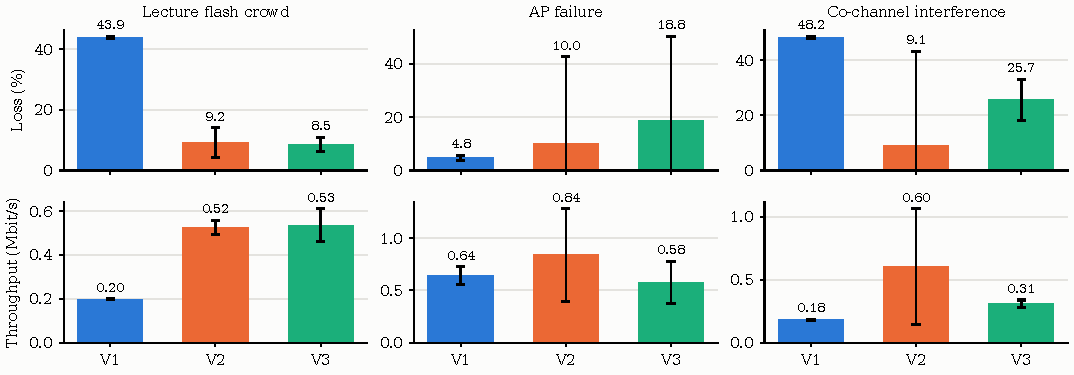
\includegraphics[width=\textwidth]{figures/fig_kpis.pdf}
\caption{Loss (top) and throughput (bottom) of the affected flows per scenario and variant; bars are means, whiskers the 95\% interval over three seeds.}
\label{fig:kpis}
\end{figure*}

\begin{figure}[t]
\centering
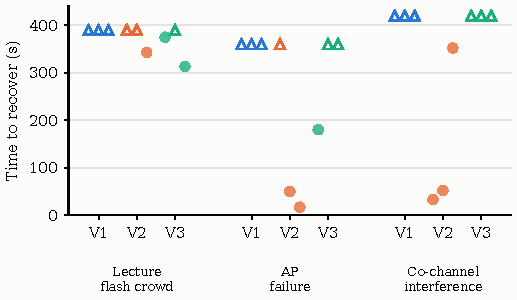
\includegraphics[width=\columnwidth]{figures/fig_recovery.pdf}
\caption{Time to recover of every run. A hollow triangle is a run that never recovered, plotted at its run end.}
\label{fig:recovery}
\end{figure}

\textbf{H1 is inconclusive in all three scenarios.} V3 is faster than V1 by \HoneFasterFlash\%, \HoneFasterApFail\% and \HoneFasterCochan\% (flash crowd, AP failure, interference; target 30\%), but plain SDN never recovered in any of its nine runs (Fig.~\ref{fig:recovery}), so each V1 time is only a lower bound.

\subsection{Safety and the twin's role (H2)}
Table~\ref{tab:actions} gives what became of every action, from the executor ledgers of the passed runs. The twin rejected \SafeVtwoAppliedTwinRejected{} actions that V2 applied anyway, \SafeVtwoHarmfulTwinRejected{} of which the watch then rolled back, and rejected \LedVthreeRejected{} in V3, none of which reached the network: the twin does block actions that would have hurt, so \textbf{H2 holds}. But it blocked few. Most harmful actions were ones it had \emph{accepted}: \SafeVtwoSlippedPastTwin{} in V2 and \SafeVthreeSlippedPastTwin{} in V3 were applied and then rolled back. Counting only those, the twin rejected \SafeVtwoHarmfulTwinRejected{} harmful actions while \the\numexpr\SafeVtwoSlippedPastTwin+\SafeVthreeSlippedPastTwin\relax{} got past it. The twin predicts the steady state after a change, not the transient in the first seconds, and only its throughput prediction was validated. The main protection was therefore the watch-and-rollback step, and it is not guaranteed: \RbFailAll{} of \the\numexpr\SafeVtwoApplied+\SafeVthreeApplied\relax{} applied actions could not be rolled back. In V3 every applied action had an accepted verdict and no high-impact change was applied without an operator (V2: \SafeVtwoHighImpactUnapproved{} such changes), which is also why V3 could not repair the interference unattended; \LedVthreeWaiting{} accepted changes were still waiting for approval when their runs ended.

\begin{table}[t]
\caption{Fate of every action in the passed runs (nine runs per variant), from the executor ledgers.}
\label{tab:actions}
\centering
\begin{tabular}{@{}lrrr@{}}
\toprule
Actions & V1 & V2 & V3 \\
\midrule
Proposed & 0 & 64 & 65 \\
Kept & 0 & 38 & 33 \\
Rolled back & 0 & 22 & 18 \\
Rollback failed & 0 & 1 & 2 \\
Still watched & 0 & 3 & 0 \\
Rejected by the twin & 0 & 0 & 4 \\
Awaiting an operator & 0 & 0 & 8 \\
\bottomrule
\end{tabular}

\end{table}

\subsection{Twin accuracy, LLM and detection}
\emph{Twin.} On \TwinN{} held-out situations (\TwinSteadyN{} of them steady-state video) the twin's mean absolute percentage error for per-flow throughput is \TwinMape\%: \TwinSteadyVideo\% in steady state, \TwinSteer\% after client steering and \TwinChannel\% after a channel change (only \TwinChannelN{} cases), while bulk TCP flows are weakest (\TwinBulkLow--\TwinBulkHigh\%). A prediction takes a median \SimMedianMs\,ms. \emph{LLM (H3).} On a 30-intent test set the cloud model translated \IntCloudOk{} of \IntCases{} correctly (median \IntCloudSeconds\,s) and the local fallback \IntLocalOk{} of \IntCases{} (median \IntLocalSeconds\,s), so \textbf{H3 holds}; every output passes the schema before the compiler sees it, and no invalid output reached the network. On live faults the copilot answered \GenCopilotOk{} of \GenCopilotN{} diagnostic questions correctly, the explainer diagnosed \GenRcaOk{} of \GenRcaN{} faults from the first alert, and all \GenActionsVerdict{} of \GenActions{} LLM-proposed actions have their twin verdict in the audit log. \emph{Detection.} The Isolation Forest reaches precision \AnoPrecision, recall \AnoRecall{} and F1 \AnoF{} on the test split and flags the AP failure \AnoDelayFail\,s after it occurs. Holt's trend method does not beat the moving average (RMSE \FcHoltOne{} against \FcMaOne{} at one minute, \FcHoltThree{} against \FcMaThree{} at three), because load changes in steps; the loop therefore reacts to measured load rather than to the forecast.

\section{Limitations}
The network is emulated on one machine with a fixed propagation model, and the numbers describe this emulation, not a real campus. The twin is calibrated on this testbed and does not predict transients. With three seeds the intervals are wide, and the evaluation seeds reuse the seed numbers of the calibration dataset, though the runs are separate and the controller acts in them. The campaign was unattended, so V3 never applied a high-impact action; with an operator its behaviour would differ. Two fixes follow from the failures: a rollback should never target an AP that is down, and the watch should not judge an action while an outside event is unfolding.

\section{Conclusion}
Used as a gate, the twin kept every applied action behind an accepted verdict and every high-impact change behind an operator, and an LLM behind that gate stated goals in natural language without ever acting on its own: no invalid output reached the network. That the twin makes control \emph{safer in outcome} is only partly shown: it blocked few harmful actions, most harmful ones were accepted, the watch-and-rollback step did most of the protecting, and in the AP-failure scenario V3's flows fared worse than plain SDN's. Whether the loop recovers the network faster depends on the fault and on having an operator for the changes that matter most; H1 could not be shown, and the evidence is mixed. We measured each failure instead of assuming it: the steers that hurt, the rollbacks that failed and the changes left waiting. Next steps are a rollback that avoids failed APs, a learned twin for bulk flows and transients, and an evaluation with an operator in the loop on real access points.

\section*{Acknowledgment}
Parts of the code and of the text were drafted with the help of an AI coding assistant (Claude Code). The authors reviewed all content and take responsibility for it.

\bibliographystyle{IEEEtran}
\bibliography{references}

\end{document}
